\documentclass[11pt,hyperref={bookmarks=false},aspectratio=169]{beamer}
\usetheme{default}
\usefonttheme{professionalfonts}
\setbeamertemplate{navigation symbols}{}
\setbeamertemplate{footline}[frame number]
\setbeamersize{text margin left=0.8cm,text margin right=0.8cm}
\usepackage{graphicx}
\usepackage{amsmath,amssymb}
\usepackage{booktabs,array}
\usepackage{tikz}
\usetikzlibrary{arrows.meta,positioning,fit}
\usepackage{enumitem,xcolor}
\setlist[itemize,1]{label=$\blacktriangleright$}
\setlist[itemize,2]{label=$\bullet$}
\setlist[itemize]{font=\color{blue}}
\setlist[enumerate,1]{label=\arabic*.}
\setlist[enumerate]{font=\color{blue}}
\setlist{itemsep=3pt,topsep=2pt,parsep=0pt}
\definecolor{tblue}{rgb}{0.2,0.2,0.7}
\newcommand{\yes}{\textcolor{green!45!black}{\checkmark}}
\newcommand{\no}{\textcolor{red!75!black}{$\times$}}

\title{Spatial Model Update}
\subtitle{The Allocation of Teaching Talent and Human Capital Accumulation}
\author{Ananth Seshadri, Simeon Alder, and Yulia Dudareva}
\date{October, 2026}

\begin{document}

\begin{frame}
  \titlepage
\end{frame}

% ---------------------------------------------------------------------------
\begin{frame}
\frametitle{The spatial model overview}
\small
\begin{columns}[T]
\begin{column}{0.45\textwidth}
\textcolor{tblue}{\textbf{Kept from the aspatial model}}
\begin{itemize}
  \item OLG with time ($s$) and goods ($e$) investment
  \item Roy choice over 21 occupations
  \item $h = h_T^{\beta}\,a^{\alpha}s^{\phi}e^{\eta}N(h_T)^{-\sigma}$, efficient class sizes
  \item Teacher pay $\kappa h^{\gamma}$, $\gamma<1$; gender wedges
\end{itemize}
\end{column}
\begin{column}{0.51\textwidth}
\textcolor{tblue}{\textbf{New}}
\begin{itemize}
  \item Ability $a_i = z\,\epsilon_i$, with $z$ inherited
  \item Two locations with local teacher markets and budgets
  \item Location choice with a moving cost
  \item Altruism: parents choose their children's schools
\end{itemize}
\end{column}
\end{columns}
\vfill
\centering
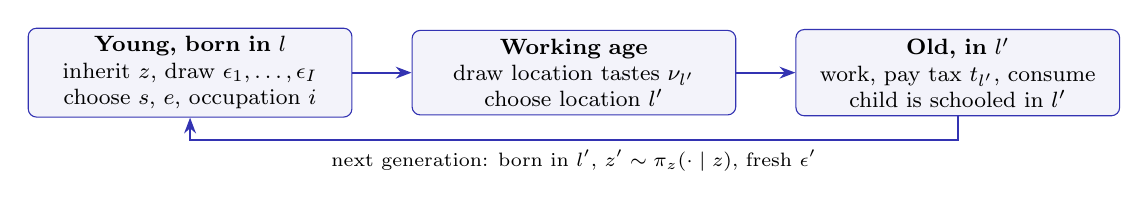
\begin{tikzpicture}[
  stage/.style={draw=tblue, fill=tblue!6, rounded corners=3pt, align=center,
                font=\footnotesize, text width=3.9cm, minimum height=1.05cm, inner sep=3pt},
  arr/.style={-{Stealth[length=2mm]}, thick, tblue}]
\node[stage] (y) {\textbf{Young, born in $l$}\\ inherit $z$, draw $\epsilon_1,\dots,\epsilon_I$\\ choose $s$, $e$, occupation $i$};
\node[stage, right=0.75cm of y] (w) {\textbf{Working age}\\ draw location tastes $\nu_{l'}$\\ choose location $l'$};
\node[stage, right=0.75cm of w] (o) {\textbf{Old, in $l'$}\\ work, pay tax $t_{l'}$, consume\\ child is schooled in $l'$};
\draw[arr] (y) -- (w);
\draw[arr] (w) -- (o);
\draw[arr] (o.south) -- ++(0,-0.3) -| (y.south)
  node[pos=0.25, below, font=\scriptsize, text=black]
  {next generation: born in $l'$, $z'\sim\pi_z(\cdot\mid z)$, fresh $\epsilon'$};
\end{tikzpicture}
\vspace{2pt}
\end{frame}

% ---------------------------------------------------------------------------
\begin{frame}
\frametitle{Ability: inherited $z$, occupation-specific $\epsilon$}
\[
a_i = z\,\epsilon_i, \qquad
\log z' = \rho_z\log z + \sigma_\xi\,\xi, \qquad
\log\epsilon_i \overset{\text{iid}}{\sim} N\!\big(-\tfrac{1}{2}\sigma_\epsilon^2,\ \sigma_\epsilon^2\big)
\]
\begin{itemize}
  \item $z$ is inherited $\Rightarrow$ families can sort across locations on $z$;
        $\epsilon_i$ is redrawn $\Rightarrow$ Roy selection
  \item Teaching pays $\kappa h^{\gamma}$, $\gamma<1$: $z$ does not cancel
        $\Rightarrow$ high-$z$ agents select out of teaching
  \item Elsewhere $z$ and location cancel, and test scores load on $z$ only
        $\Rightarrow$ estimate outside equilibrium:
\end{itemize}
\medskip
\centering
\footnotesize
\renewcommand{\arraystretch}{1.15}
\begin{tabular}{@{}llrr@{}}
\toprule
Parameter & Target & Data & Estimate \\
\midrule
Occupational dispersion $\sigma_\epsilon$ & Within-occupation wage 90/10 (ACS) & 3.74 & 0.786 \\
Persistence $\rho_z$ & Mother--child latent score corr.\ (CNLSY) & 0.577 & 0.577 \\
Dispersion of $z$, $s_z$ & Log wage per latent AFQT SD (NLSY79) & 0.213 & 0.196 \\
\bottomrule
\end{tabular}
\end{frame}

% ---------------------------------------------------------------------------
\begin{frame}
\frametitle{Two locations with local teacher markets}
\centering
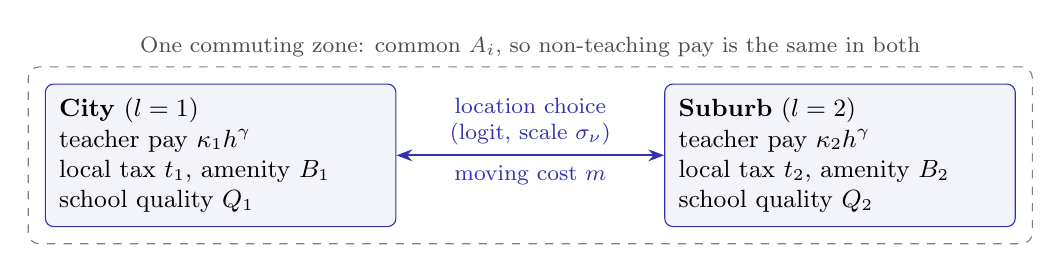
\begin{tikzpicture}[
  loc/.style={draw=tblue, fill=tblue!6, rounded corners=3pt, align=left,
              font=\small, text width=4.1cm, inner sep=5pt},
  arr/.style={{Stealth[length=2mm]}-{Stealth[length=2mm]}, thick, tblue}]
\node[loc] (c) {\textbf{City} ($l=1$)\\ teacher pay $\kappa_1 h^{\gamma}$\\ local tax $t_1$, amenity $B_1$\\ school quality $Q_1$};
\node[loc, right=3.4cm of c] (s) {\textbf{Suburb} ($l=2$)\\ teacher pay $\kappa_2 h^{\gamma}$\\ local tax $t_2$, amenity $B_2$\\ school quality $Q_2$};
\draw[arr] (c) -- node[above, font=\footnotesize, align=center] {location choice\\(logit, scale $\sigma_\nu$)}
                  node[below, font=\footnotesize] {moving cost $m$} (s);
\node[draw=gray, dashed, rounded corners, fit=(c)(s), inner sep=6pt,
      label={[font=\footnotesize, text=black!70]above:One commuting zone: common $A_i$, so non-teaching pay is the same in both}] {};
\end{tikzpicture}
\raggedright
\begin{itemize}
  \item School quality $Q_l = \big(2\widetilde H_{T,l}/M_l\big)^{\sigma}$: local teacher human
        capital per pupil
  \item Teachers are paid from a local balanced budget; class size is the only congestion force
  \item Baseline: live $=$ work $=$ school. Equilibrium is a fixed point in
        $(\widetilde H_{T,l}, M_l, t_l)$ with a stationary $\Phi_l(z)$
\end{itemize}
\end{frame}

% ---------------------------------------------------------------------------
\begin{frame}
\frametitle{Altruism and the sorting problem}
\[
U = \ln(1-s) + \mathbb{E}\big[\,\mu\ln C + B_{l'} + \sigma_\nu\nu_{l'} + \lambda f(h')\,\big],
\qquad h' = \text{child's human capital}
\]
\begin{itemize}
  \item Parents do not fund the child's investment, so location $l'$ is worth
  \[
  V_{l'} = \mu\ln C_{l'} + \Lambda_{l'}(z), \qquad
  \Lambda_{l'}(z) = \lambda\,\mathbb{E}\big[f(h')\mid z,\,l'\big]
  \]
  $\Rightarrow$ altruism acts \alert{only through location choice}
  \item \textbf{Neutrality:} with $f=\log$ and a utility moving cost, location premia are
        proportional $\Rightarrow$ no sorting on ability
  \item Two departures, no new free parameters:
  \begin{enumerate}
    \item \textbf{Goods moving cost} $m = r_m\bar C$: weighs more on the poor
    \item \textbf{Linear warm glow} $f(h') = h'/\bar h - 1$: schools matter more for abler children
  \end{enumerate}
\end{itemize}
\end{frame}

% ---------------------------------------------------------------------------
\begin{frame}
\frametitle{Data: city vs.\ suburb within a commuting zone}
\begin{columns}[c]
\begin{column}{0.40\textwidth}
\small
\begin{itemize}
  \item City (NCES 11--13) vs.\ suburban (21--23) districts, 188 CZs
  \item Moments: within-CZ gaps, enrollment-weighted
\end{itemize}
\bigskip
Schools look alike; families do not $\Rightarrow$ the gap is mostly \alert{who lives there}
\end{column}
\begin{column}{0.56\textwidth}
\footnotesize
\renewcommand{\arraystretch}{1.12}
\begin{tabular}{@{}lr@{}}
\toprule
Suburb $-$ city & Gap (SE) \\
\midrule
\multicolumn{2}{@{}l}{\textcolor{tblue}{\textit{Schools}}} \\
Teacher salary, log$^\dagger$ & 0.009 (0.009) \\
Teachers per pupil, log & $-$0.018 (0.013) \\
SEDA learning rate, SD/grade & 0.003 (0.003) \\
\multicolumn{2}{@{}l}{\textcolor{tblue}{\textit{Families}}} \\
Median FTYR earnings, log & 0.112 (0.017) \\
Child poverty, pp & $-$8.9 (0.9) \\
SEDA score level, SD & 0.289 (0.033) \\
\midrule
Enrollment, log$^\dagger$ & 0.376 (0.115) \\
City$\leftrightarrow$suburb move rate$^\dagger$ & 0.216 (0.011) \\
\bottomrule
\end{tabular}

\smallskip
$^\dagger$ targeted in the calibration
\end{column}
\end{columns}
\vfill
\scriptsize
Sources: CCD, F-33, CWIFT, SAIPE, ACS (districts, 2018); SEDA 2009--19; NLSY79 (move rate).
\end{frame}

% ---------------------------------------------------------------------------
\begin{frame}
\frametitle{Calibration: eight parameters in equilibrium}
\small
Fixed: $\sigma=0.56$ (class size, FOO), $\sigma_\nu=0.25$ (Eckert--Kleineberg),
$\chi=\log 1.12$ (CFR). First stage: $A_i$ and female wedges match occupation shares by gender.\par
\medskip
\centering
\footnotesize
\renewcommand{\arraystretch}{1.15}
\begin{tabular}{@{}lrllr@{}}
\toprule
Parameter & Value & Target & Source & Data \\
\midrule
Pay scale $\log\tilde\kappa$ & $-$1.204 & Male teaching share & ACS & 1.95\% \\
Female outside option $\omega_f$ & 0.966 & Female teaching share & ACS & 5.99\% \\
Teacher wage curvature $\gamma$ & 0.619 & Teachers' wage 90/10 & ACS & 2.77 \\
Suburb pay premium $\delta_\kappa$ & 0.0045 & Salary gap & F-33 & 0.0086 \\
Suburb amenity $\Delta B$ & 0.066 & Enrollment gap & CCD & 0.376 \\
Teacher spillover $\beta$ & 0.228 & Earnings per SD-year of teacher quality & CFR & 1.34\% \\
Altruism $\lambda$ & 0.125 & WTP for school scores, \% of $C$ & BFM & 0.60\% \\
Moving cost $r_m$ & 0.206 & City$\leftrightarrow$suburb move rate & NLSY79 & 0.216 \\
\bottomrule
\end{tabular}\par
\medskip
\raggedright
\small
\begin{itemize}
  \item Exactly identified: all eight matched; 15 dispersed starts find no other root
  \item Jacobian full rank (condition number 30); each spatial moment loads on its own parameter
\end{itemize}
\end{frame}

% ---------------------------------------------------------------------------
\begin{frame}
\frametitle{Validation: the fit misses sorting and teacher allocation}
\begin{columns}[T]
\begin{column}{0.56\textwidth}
\footnotesize
\setlength{\tabcolsep}{4pt}
\renewcommand{\arraystretch}{1.1}
\begin{tabular}{@{}lrr@{}}
\toprule
Untargeted moment & Data & Model \\
\midrule
\multicolumn{3}{@{}l}{\textcolor{tblue}{\textit{Household sorting}}} \\
Earnings gap, log & 0.112 & $-$0.010 \\
SEDA score gap, SD & 0.289 & 0.061 \\
Child-poverty gap, pp & $-$8.9 & $+$0.2 \\
City share, top $-$ bottom tercile & $-$0.295 & $+$0.011 \\
\multicolumn{3}{@{}l}{\textcolor{tblue}{\textit{Teacher allocation}}} \\
Teachers-per-pupil gap, log & $-$0.018 & $+$0.023 \\
Learning-rate gap, SD/grade & 0.003 & 0.012 \\
\multicolumn{3}{@{}l}{\textcolor{tblue}{\textit{Teacher selection}}} \\
Teacher / non-teacher schooling & 1.18 & 0.76 \\
Teachers' ability vs.\ others, SD & $+$0.61 & $-$0.29 \\
Teacher pay vs.\ market, m/f & $+$.06/$+$.09 & $-$.72/$-$.63 \\
\bottomrule
\end{tabular}
\end{column}
\begin{column}{0.40\textwidth}
\small
\begin{itemize}[itemsep=8pt]
  \item \textbf{No sorting:} the suburb's school edge is worth $\le 0.002$ utils vs.\
        $\sigma_\nu = 0.25$; WTP pins $\lambda$, SEDA growth keeps $\Delta\log Q$ small
  \item \textbf{Over-staffing:} matching the small pay gap over-staffs the suburb and
        inflates its learning-rate edge
  \item \textbf{Negative selection:} with $\gamma<1$, high-$z$ agents avoid teaching;
        short schooling fills it at low pay
\end{itemize}
\end{column}
\end{columns}
\end{frame}


% ---------------------------------------------------------------------------


\end{document}
